\documentclass{article}
\usepackage{spconf,amsmath,amssymb,graphicx}
\usepackage[utf8]{inputenc}
\usepackage{xspace}
\usepackage{graphicx}
\usepackage[dvipsnames]{xcolor}
\usepackage[ruled]{algorithm2e}
\usepackage{balance}
\usepackage{url}

%%%%%%%%%%%%%%%%%%%%%%%%%%%%%%%%%%%%%%%%%%%%%%%%%%%%%%%%%%%%%%%%%%%%%%%%%%%
% version control
%%%%%%%%%%%%%%%%%%%%%%%%%%%%%%%%%%%%%%%%%%%%%%%%%%%%%%%%%%%%%%%%%%%%%%%%%%%
%
%\definecolor{NewTextFG}{rgb}{0.0,0.3,0.5}
\definecolor{NewTextFG}{rgb}{0.0,0.1,0.2}
\newcommand{\fix}{\marginpar{FIX}}
\newcommand{\pendcite}[1]{{\color{red}[#1]}}
%\newcommand{\note}[1]{\colorbox{yellow}{\scriptsize NOTE: #1}} % a la Acrobat
\newcommand{\newtext}[1]{{\color{NewTextFG}{#1}}\xspace}
\newenvironment{textnote}[1]{\colorbox{yellow}{\scriptsize #1$\gg$}}{\colorbox{yellow}{\scriptsize $\ll$}\xspace}
\newcommand{\best}[1]{\textbf{\color{blue}#1}\xspace}
%\newcommand{\mnote}[1]{\marginpar{\framebox{\bf#1}}}
%\newcommand{\ok}[1]{\marginpar{\framebox{\large\color{blue}\checkmark}}}
\newcommand{\mnote}[1]{}
\newcommand{\ok}[1]{}

%
%%%%%%%%%%%%%%%%%%%%%%%%%%%%%%%%%%%%%%%%%%%%%%%%%%%%%%%%%%%%%%%%%%%%%%%%%%%
% Conventions
%%%%%%%%%%%%%%%%%%%%%%%%%%%%%%%%%%%%%%%%%%%%%%%%%%%%%%%%%%%%%%%%%%%%%%%%%%%
%
\newcommand{\iter}[1]{^{(#1)}}
\newcommand{\BlackBox}{\rule{1.5ex}{1.5ex}}  % end of proof
\newenvironment{proofi}{\par\noindent{\bf Proof: }}{\hfill\BlackBox\\}
\def\opt{\ensuremath{^{*}}}
\providecommand{\argmin}{\mathop{\textup{argmin}}}
\def\gradient{\nabla}
\def\hessian{\nabla^2}
\def\reals{\ensuremath{\mathbb{R}}}
\def\naturals{\ensuremath{\mathbb{N}}}
\newcommand{\mxn}{m{\times}n}
\renewcommand{\vec}[1]{\ensuremath{\mathbf{\MakeLowercase{#1}}}}
\newcommand{\mat}[1]{\ensuremath{\mathbf{\MakeUppercase{#1}}}}
\newcommand{\rv}[1]{\ensuremath{\MakeUppercase{#1}}}
\newcommand{\dpdf}[1]{\mathrm{\ensuremath{\MakeUppercase{#1}}}}
\newcommand{\cpdf}[1]{\mathrm{\ensuremath{\MakeLowercase{#1}}}}
\newcommand{\st}{\ensuremath{\mathrm{s.t.}}}
\newcommand{\norm}[1]{\ensuremath{\left\|#1\right\|}}
\newcommand{\quant}[1]{\ensuremath{\left[#1\right]}}
\newcommand{\support}[1]{\mathrm{supp}(#1)}
\newcommand{\rankf}[1]{\mathrm{rank}(#1)}
\def\rank{\mathrm{rank}}
\newcommand{\fun}[1]{\mathrm{#1}}
\newcommand{\cost}[1]{\ensuremath{\ell_{#1}}\xspace}
\newcommand{\abs}[1]{\ensuremath{\left|#1\right|}}
\newcommand{\setdef}[1]{\ensuremath{\left\{#1\right\}}}
\newcommand{\vecdef}[1]{\ensuremath{\left(#1\right)}}
\newcommand{\setspan}{\ensuremath{\mathrm{span}}}
\newcommand{\svec}[1]{_{[#1]}}
\def\transp{^\intercal}
\newcommand{\refeq}[1]{(\ref{#1})}
\def\med{\ensuremath{\mathrm{med}}}
\newcommand{\col}[1]{_{#1}}
\newcommand{\row}[1]{^{#1}}
\def\Ident{\mat{I}}
\def\Risk{\ensuremath{\oR}}
\def\Loss{\ensuremath{\ell}}
\def\Gaussian{\ensuremath{\mathcal{N}}}
\newcommand{\GaussianPDF}[2][\sigma]{\ensuremath{\frac{1}{\sqrt{2\pi#1^2}}e^{-\frac{#2^1}{2#1^2}} }}
\def\Exponential{\ensuremath{\mathrm{Exp}}}
\def\Bernoulli{\ensuremath{\mathrm{Ber}}}
\def\Laplacian{\ensuremath{\mathrm{Lap}}}
\newcommand{\LaplacianPDF}[2][\vv]{\ensuremath{\frac{1}{2#1}e^{-\frac{|#2|}{#1}} }}
\def\Indicator{\ensuremath{\mathbf{1}}}
\def\LG{\ensuremath{\mathrm{LG}}}
\def\MOEG{\ensuremath{\mathrm{MOEG}}}
\def\MOE{\ensuremath{\mathrm{MOE}}}
\def\sgn{\mathrm{sgn}}
\newcommand{\minimize}{\ensuremath{\mathrm{minimize}\quad}}
\newcommand{\maximize}{\ensuremath{\mathrm{maximize}\quad}}
\def\defeq{:=}
\def\assign{\leftarrow}
\newcommand{\spaze}[1]{\ensuremath{\mathbb{#1}}}
\newcommand{\inva}[1]{\left(#1\right)^{-1}}
\def\inv{^{-1}}
\newcommand{\pinva}[1]{\left(#1\right)^{\dagger}}
\def\pinv{^{\dagger}}
%
% data
%
\def\patdim{m}
\def\patnum{n}
\def\projnum{k}
\def\sigdim{N}
\def\sigspace{\reals^{\sigdim}}
\def\patspace{\reals^{\patdim}}
\def\patmspace{\reals^{\patdim{\times}\patnum}}
\def\dictmspace{\reals^{\ndims{\times}\dicdim}}
\def\coefmspace{\reals^{\dicdim{\times}\patnum}}
\def\dictmspace{\reals^{\ndims{\times}\natoms}}
\newcommand{\acro}[1]{\MakeUppercase{#1}\xspace}
\def\admm{\acro{admm}}
\def\paco{\acro{paco}}
\def\pave{\acro{pave}}
\def\dct{\acro{dct}}
\def\bcs{\acro{bcs}}
%
\def\zeros{\mat{0}}
\def\ident{\mat{I}}
\def\ones{\mat{1}}
\def\mX{\mat{X}}
\def\mR{\mat{R}}
%\def\oR{\mathcal{R}}
\def\va{\vec{a}}
\def\vb{\vec{b}}
\def\ve{\vec{e}}
\def\vu{\vec{u}}
\def\vv{\vec{v}}
\def\vw{\vec{w}}
\def\vx{\vec{x}}
\def\vy{\vec{y}}
\def\vz{\vec{z}}
\def\vt{\vec{t}}
\def\vs{\vec{s}}

\def\mP{\mat{P}}
\def\mY{\mat{Y}}
\def\mZ{\mat{Z}}
\def\mU{\mat{U}}
\def\mD{\mat{D}}
\def\mW{\mat{W}}
\def\mA{\mat{A}}
\def\mB{\mat{B}}
\def\hy{\hat{y}}
\def\hx{\hat{x}}
\def\hmA{\hat{\mA}}
\def\hmY{\hat{\mY}}
\def\hva{\hat{\va}}
\def\hvx{\hat{\vx}}
\def\hvy{\hat{\vy}}
\def\tvv{\tilde{\vv}}
\def\tvx{\tilde{\vx}}
\def\tvy{\tilde{\vy}}
\def\tmY{\tilde{\mY}}
%\def\oS{\mathcal{S}}
\def\ost{\mathcal{S}}
\def\spX{\mathbb{R}^N}
\def\spY{\mathbb{R}^{mn}}
\def\spC{\mathbb{C}}
\def\vecop{\mathrm{vec}}
\def\matop{\mathrm{mat}}
\def\tv{\mathrm{TV}}
\def\opR{\mathcal{R}}
\def\opS{\mathcal{S}}
\def\llbracket{[\![}
\def\rrbracket{]\!]}
\newcommand{\proj}[1]{\ensuremath{\llbracket{#1}\rrbracket}}

\def\projOp{\mathrm{\Pi}}
%\newcommand{\prox}[2]{\ensuremath{\mathrm{prox}_{#1}\left(#2\right)}}
\def\prox{\mathrm{prox}}
\def\vone{\mathbf{1}}

\def\ladmm{\acro{ladmm}}

\def\tmV{\tilde{\mat{V}}}
\def\ball{\mathcal{B}}

\newcommand{\note}[1]{\color{red}#1\color{black}}

\def\vq{\vec{q}}

\title{Practical Bulk Denoising of Large Binary Images}

\name{Ignacio Ramírez Paulino}
\address{%
  Universidad de la República\\
  Instituto de Ingeniería Eléctrica \\
  Julio Herrera y Reissig 565, Montevideo, Uruguay \\
  nacho@fing.edu.uy}

\begin{document}

\maketitle

\begin{abstract}
This paper explores the problem of removing real, non-simulated noise from a large body of large binary images. Three denoising methods are evaluated for their efficacy and speed: the well known DUDE, a novel variant of it which we call the Quorum Denoiser, and an adaptation of the Non-Local Means (NLM) method for binary images, B-NLM which, to our knowledge, is faster than other known variants. The methods are compared and tested both on simulated noise (as a benchmark) and on the real life images. All three methods produce good results on real noise. However, despite being optimized, the B-NLM is significantly slower than the other two, whose speeds are comparable to a plain median filter. Overall, the Quorum denoiser appears to be the best option, both in quality (real and simulated) and speed.
\end{abstract}

\begin{keywords}
image denoising, binary image denoising, DUDE, non-local means, real noise
\end{keywords}

%
%===============================================================================
\section{Introduction}
%===============================================================================
%
\label{sec:intro}
% PARA ARXIV “© 20XX IEEE. Personal use of this material is permitted. Permission from IEEE must be obtained for all other uses, in any current or future media, including reprinting/republishing this material for advertising or promotional purposes, creating new collective works, for resale or redistribution to servers or lists, or reuse of any copyrighted component of this work in other works.”
Binary images have received little attention from the image processing community; this applies in particular to the problem of binary image denoising. However, and contrary to what one might expect, removing noise from binary images can be considerably more challenging than doing so from grayscale or color images. Intuitively, there is no continuity to cling onto as when removing, say, Gaussian noise, which is the basic assumption of most denoising algorithms. Also, the noisy samples take on the same two values as the clean samples and  telling them apart is not easy. \\

More formally, the capacity on the binary symmetric channel (BSC) with error rate $p=0.1$ is $1-h(p)$,  where $h(p)=-p\log p-(1-p)\log (1-p)$ is the binary entropy function. This means that, when a signal $\vx$ passes through a BSC, the proportion of information that is lost is $h(p)$ bits per symbol. For example, for $p=10\%$ (which might not seem much), \emph{this amounts to $\sim 50\%$ of the information being lost!} Adding to the  potential confusion, the BSC could be interpreted as the ``binary version'' of the well known ``Salt \& Pepper'' (S\&P) noise. Yet, the same 10\% error rate of S\&P noise on an 8-bit grayscale image reduces the information by a mere 10\% (approximately), or 3\% on 24 bit color images. 

On the other hand, there are significant advantages in working directly with the binary information. First, accurate noise models specific to binary random variables can be used for inference. Second, huge computational savings can be obtained by working with bit-valued samples instead of float-valued ones; in the real life case that motivates this work~\cite{luisa}, which involves several millions of very large binary images (15--20 megapixel), such savings make the difference between processing the whole batch in a couple of days or a whole year. 

A sad testimony to the lack of interest in binary image processing is the scarce literature on the topic. Only a handful of novel methods have been developed over the last 20 years~\cite{dude-bin,shift-denoising,compression-denoising,mcmc-denoising}. Most of these are derived from the DUDE~\cite{dude-bin}, a powerful method with a solid theoretical foundation. The latest development in this direction is the so called Neural DUDE~\cite{neural-dude}.
Prior to that, the standard for binary image denoising was to use morphological operators (see e.g. ~\cite{morph}). 

Meanwhile, denoising methods for continuous-valued images have been a mainstream topic in image processing for over 30 years. A wealth of methods and families of methods, notoriously non-local means~\cite{nlm}, non-local Bayes (NLB)~\cite{nlbayes}, BM3D~\cite{bm3d}, EPLL~\cite{epll}, and Deep Learning-based denoising (FFDNet)~\cite{deep-learning} have each pushed the boundaries of what was possible in this field. Thus, no work on this subject should omit a study of at least some of the state of the art methods described above. However, adapting such methods to the binary case can be quite challenging. For instance, it is not trivial to translate the inference methods used for Gaussian sources and noise (such as in EPLL, BM3D and NLB) to the binary case. The only exception is non-local means~\cite{nlm}, which is quite easy to adapt. As for the others, not only they perform terribly on non-Gaussian noise: even methods considered fast such as BM3D and FFDNet require orders of magnitude more to run on our images than the ones we discuss below. 

\subsection{Contributions}

According to the above discussion, we evaluate three methods for binary image denoising: the  DUDE~\cite{dude-bin}, a novel variant called Quorum Denoiser, and a binary adaptation of Non-Local Means.  The DUDE is implemented and applied as described in~\cite{dude-bin}, albeit with a better context model than the one described there. The Quorum Denoiser replaces the full context description used in DUDE by a simple statistic of it. This leads to improvements both in speed and performance (especially on real noise where the DUDE breaks down).

We also adapt the non-local means algorithm~\cite{nlm} so that neighborhood distances are efficiently computed in terms of bit-wise operations. A special neighborhood shape allows us to avoid a weighted distance while retaining the desirable locality properties of the comparison (this will be made clear later). The resulting adaptation requires significantly time than the fastest reported non-local means variants~\cite{fast-nlm}.

%And last, for something completely different, we propose and evaluate a method for accurate estimation of the two noise rates of non-symmetric binary noise. This is a crucial step for the DUDE and Quorum denoisers, which require a good estimation of these parameters.


%=============================================================================
\section{Preliminaries}
%=============================================================================
An image $\vx$ is represented as a $m{\times}n$ array of binary values indexed by a pair of integers $(i,j) \in \Omega$ so that $x_{ij}$ is the pixel value at row $i$ and column $j$, and $\Omega = [0,m-1]\times[0,n-1] \subset \mathbb{N}^2$. We use $\vx$ to refer to the \emph{clean, unobserved} image to be recovered, $\vz$ to its observed, noisy version, and $\hvx$ to an estimation of $\vx$ obtained by some denoising method. The image samples take values in an alphabet $A=\{0,\ldots,\alpha-1\}$. For binary images, $\alpha=2$.
\def\hx{\hat{x}}
\def\vb{\vec{b}}
The methods discussed in this work belong to the family of neighborhood filters, in the sense that each element in the denoised image, $\hx_{i,j}$, is a function of the corresponding neighboring pixels in the noisy image, and their center, $z_{i,j}$. The neighborhood relationship is defined by means of a \emph{template}. A template $T$ is a set of $k$ \emph{relative} 2D indexes: $(\delta,\lambda) \in \mathbb{Z}$: $T=\{(\delta_1,\lambda_1),(\delta_2,\lambda_2),\ldots,(\delta_k,\lambda_k)\}$. The neighborhood of  pixel $x_{i,j}$ as defined by $T$ is a vector of sample values $\vb_{i,j}=\{x_{i+\delta,j+\lambda}: (\delta,\lambda) \in T\}.$ To fix ideas, a typical template is the $\ell_\infty$ ball of radius $r$, for example with $r=3$, giving rise to $7{\times}7$ square neighborhoods centered at the ``target'' pixel $x_{i,j}$.
Square neighborhoods are usually called \emph{patches}. Since most neighborhood-based methods have been developed using square neighborhoods, they are often called \emph{patch-based methods}. However, nothing prevents these methods from being applied to  neighborhoods defined by arbitrary templates.

The random variables $X,\,Z \in A$ represent generic clean and noisy samples respectively. Likewise, $B \in A^k$ is a $k$-dimensional random variable representing a generic neighborhood (also called a ``context''). 

%==============================================================================
\section{The DUDE} 
%==============================================================================
\label{sec:bdude}
\def\Pr{\ensuremath{\mathrm{Pr}}}
\def\ti{^{-T}}
The Discrete Universal DEnoiser (DUDE)~\cite{dude} is a general framework for denoising discrete-valued, discrete-time, arbitrary dimensional signals. The DUDE is a two-pass algorithm with four inputs: the input image $\vz$ which takes values in a discrete alphabet $\{0,\ldots,\alpha-1\}$ a template $T$, a loss function $\Lambda=\{\ell_{i,j}:i,j \in A\}$ indicating the loss incurred in inferring a sample value $j$ when the (unobserved) true is $i$, and a channel transition matrix $\Pi$ so that $\pi_{i,j}=\Pr(Z=j|X=i)$. The first pass collects  statistics: for each neighborhood $\vb$, its number of occurences $n(\vb)$ and the joint occurences of each $\vb$ and the center value $z$, $n(\vb,z)$, are computed (note that the templates $T$ used in the DUDE never include the center pixel, which is considered separately as described before).

During the second pass, the estimated clean samples $\hat{x}_{i,j}$ are estimated so that the empirical Bayes loss is minimized. This is given by (see~\cite{dude} for details):
\begin{equation}
\hat x_{i,j} = \arg\min_x n(\vb_{i,j},z_{i,j}) \Pi\ti [\pi_{:,z_{i,j}} \odot \ell_{:,x} ],  \label{eq:dude}
\end{equation}
where $\odot$ means element-wise product  $\pi_{:,j}$ and $\ell_{:,j}$ denote the $j$-th columns of $\Pi$ and $\Lambda$ respectively.
In our setting, we use the Hamming loss function $\ell(x,y)=\mathbf{1}_{x \neq y}$ and 
$$
\Pi = \left(\begin{array}{cc}
1-\rho_{0}     & \rho_{0} \\
\rho_1      & 1-\rho_{1}.
\end{array}\right)
$$
where $\rho_0$ and $\rho_1$ are error rates that need to be specified. Plugging $\ell$ and $\Pi$ in \refeq{eq:dude} leads to the following \emph{decision rule}:
\begin{equation}
    \left\{
    \begin{array}{ccc}
        z=0,&\frac{n(\vb,0)}{n(\vb,0)+n(\vb,1)} \geq \frac{2p_1(1-p_0)}{1+p_0-p_1}&\rightarrow \hx = 0\\
        z=0,&\frac{n(\vb,0)}{n(\vb,0)+n(\vb,1)} < \frac{2p_1(1-p_0)}{1+p_0-p_1}&\rightarrow \hx = 1\\        
        z=1,&\frac{n(\vb,1)}{n(\vb,1)+n(\vb,1)} \geq \frac{2p_0(1-p_1)}{1+p_1-p_0}&\rightarrow \hx = 1\\        z=1,&\frac{n(\vb,1)}{n(\vb,1)+n(\vb,1)} < \frac{2p0(1-p1)}{1+p_1-p_0}&\rightarrow \hx = 0\\        \end{array}
    \right.
\end{equation}

Given enough samples, the DUDE is guaranteed to match the performance of \emph{any} neighborhood denoiser. However, in order to do so, the number of samples required can be very large, and this number grows quickly with the template size and the number of samples.
Also, the noise has to be \emph{memoryless} (i.e., uncorrelated or ``white''); deviating from this hypothesis usually leads to a bad performance.
The DUDE was applied to binary images in~\cite{dude-bin}, although as a proof of concept, with experiments limited to the particular case of half-tone images. However, even with the smallest possible alphabet (binary) and several megapixel images, the DUDE becomes impractical for templates of more than, say, $20$ samples (leading to $2^{20}$ possible neighborhoods), already smaller than a $5{\times}5$ square patch. 
%The generic DUDE algorithm is given in Algorithm~\ref{alg:bdude}. 
%
%\begin{algorithm}
%\caption{\label{alg:bdude}The DUDE}
%\SetKwInOut{Input}{Input}
%\SetKwInOut{Output}{Output}
%\Input{Noisy image $\vz$; $\rho_0$; $\rho_1$; template $T$; loss fun. $\ell$ }
%\Output{Denoised image $\hvx$}
%Compute $n(\vb,z)$ for each $(\vb,z)$ occurring in $\vz$ \;
%Compute $\vq(\vb,z)[x] = n(s,z) \Pi\ti [\ell_{:,x} \odot \Pi_{:,z}] $ for each %$(\vb,z)$ in $\vz$ and $x \in A$\;
%Set $\hvx_{i,j} = \arg\min_{x\in A} \vq(s_{i,j},z_{i,j})$ for each $(i,j)$\;
%\end{algorithm}
%

\section{Quorum Denoiser}

What we propose here is similar to the strategy followed in~\cite{dude-i} to apply the DUDE to continuous-tone images: we replace  the ``raw'' contexts $\vb$ by a non-injective context statistic $S(B)$. This statistic is simply the sum of $\vb$, $s(\vb)=\sum_i b_j$, which we call the ``quorum'' of $\vb$ to avoid confusions. We then replace $n(\vb,z)$ by $n(s(\vb),z)$ in \refeq{eq:dude}, where now $n(s,z)$ counts the number of joint occurrences of the quorum value $s$ and noisy sample $z$ in the image (note: images are zero padded so that all contexts are properly defined). Algorithm~\ref{alg:quorum} summarizes this method. 

\begin{algorithm}
\caption{\label{alg:quorum}Quorum Denoiser}
\SetKwInOut{Input}{Input}
\SetKwInOut{Output}{Output}
\Input{Noisy image $\vz$; $\rho_0$; $\rho_1$; template $T$; loss fun. $\ell$ }
\Output{Denoised image $\hvx$}
\For{each $(i,j) \in \Omega$}{
$s_{i,j}\gets \sum_{(\delta,\lambda) \in T} z_{i+\delta,j+\lambda}$% for each $(i,j)$ in $\Omega$\;
}
\For{each $(s,z)$ occurring in $\vz$ and $x=0,1$}{
$\vq(s,z)[x] \gets n(s,z) \Pi\ti [\ell_{:,x} \odot \Pi_{:,z}] $
}
\For{each $(i,j) \in \Omega$}{
$\hvx_{i,j} \gets \arg\min_x \vq(s_{i,j},z_{i,j})$
}
\end{algorithm}
%==============================================================================
\section{Binary Non-local Means Denoiser} 
%==============================================================================
\label{sec:bnlm}
\def\mD{\mat{D}}
The non-local means (NLM) method in~\cite{nlm}, gave rise to  a major   non-local image processing paradigm, with several applications beyond denoising. The method is simple, elegant and powerful. Furthermore, it is straightforward to implement and adapt to our case of interest. Given a template $T$, the denoised value $\hat{x}_{i,j}$ is given by:
$$\hx_{i,j} = \sum_{i',j'} z_{i',j'} w(\,b_{i,j}\transp\mD b_{i',j'}\,)$$ 
where $w(d)$ is a non-increasing function of $d$ and $\mD$ is usually a diagonal scaling matrix which puts more weight on context samples closer to the center of the template. In words, $\hx_{i,j}$ is a weighted average of all the pixels $z_{i',j'}$ in $\vz$, where the weight is given by the similarity between the context at $(i,j)$ and the one at $(i',j')$. In the continous-valued NLM, $w(\cdot)$ is a Gaussian function with scale parameter $\sigma$ chosen by the user and $\mD$ is a diagonal matrix whose elements are also a Gaussian function of the distance of the template sample to its center. 

In our case, we can leverage from special purpose CPU instructions such as \texttt{popcount}, to count the number of $1s$ in a binary 128 bit word, or the standard bitwise \texttt{and}. If we set $\mD=\mathbf{Id}$, the weight is given by $w(h(\vb,\vb'))$ where $h(\vb,\vb')=\sum(\vb \oplus \vb')$ is the Hamming distance between $\vb$ and $\vb'$, that is, the number of places where they differ. This computation requires just \emph{two CPU instructions}: $$\sum(\vb \oplus \vb')=\mathrm{popcount}(\mathrm{and}(\vb,\vb')),$$ which is which is dramatically faster than a weighted euclidean norm computation between two floating point-valued vectors. As in~\cite{nlm}, the weight function $w(\cdot)$ can be  a Gaussian with user-selectable parameter. In our case, since there are only $k+1$ possible values of $h(\cdot)$, we can pre-compute $w$ into a lookup table instead of evaluating $w(\cdot)$ each time (toghether with $h(\cdot)$, computing $w(\cdot)$ is the most computationally-intensive part of the algorithm).
To further speed up the algorithm, we discard contexts whose distance to the target context is larger than a given value $d_{\max}=\max\{4,2(\rho_0+\rho_1)k\}$; this is how $\rho_0$ and $\rho_1$ affect the operation of B-NLM, and is equivalent to setting $w(d)=0$ for $d\geq d_{\max}$.
Algorithm \ref{alg:bnlm} summarizes the proposed implementation.

\begin{algorithm}
\caption{\label{alg:bnlm}Binary Non-Local Means}
\SetKwInOut{Input}{Input}
\SetKwInOut{Output}{Output}
\Input{Noisy image $\vz$; $\rho_0$; $\rho_1$; decay rate $\beta$; template $T$; search template $W$ }
\Output{Denoised image $\hvx$}
\For{each $(i,j) \in \Omega$}{
$h_{\delta,\lambda} \gets h(\vb_{i,j},\vb_{i+\delta,j+\lambda} ),\,\forall (\delta,\lambda) \in W$\;
$\hx_{i,j} \gets \mathrm{round}\left(\sum_{(\delta,\lambda) \in W} w(h_{\delta,\lambda})z_{i+\delta,j+\lambda}\right)$\; 
}
\end{algorithm}

%\subsection{The need for a special template}
%
%Note that there is a delicate aspect in the above choice for distances: if a full context (e.g., a patch) is used, it is important that samples away from the center weight less than those close to it. Otherwise, the unweighted distance will be dominated by the contribution of the outermost samples. For example, on a $5{\times}5$ patch, there are $16$ outer pixels and only $8$ next to the center. 

%In order for us to avoid the above problem while also avoiding a weighted distance computation, we employ a special ``star-shaped'' template whose eight rays extend to the north, east, south, west, northeast, northwest, southeast and southwest of the center, in each case a fixed number of pixels given by the template radius (for a radius of $1$, the template produces standard $3{\times}3$ patches). 

%As it turns out, this template shape also allows the DUDE to take in information from larger surrounding areas while keeping the context size small.

%Albeit much faster than the baseline implementation, even with these speedups, the binary NLM  takes $O(km^2n^2)$ operations to complete, which is still rather slow on $15--20$ megapixel images. Thus, as with the baseline NLM, the  practical application of the modified version still requires one to restrict the weighted sum to a search window around the pixel to be denoised. As we will see, even for a small search radius of $10$ (the typical value used in the original NLM), the modified NLM is significantly slower than the other two methods. 

\subsection{On the choice of the template}

Typical denoising applications use square templates centered at the ``target'' pixel. While this is a reasonable choice in general, there are two reasons for us to deviate from this default. First, the DUDE cannot work effectively with large templates. Also, since our Binary NLM algorithm considers near and far neighbor pixels alike, a full context would give too much weight to the outer pixels. What we use istead is an eight-point star-shaped context with rays extending to the north, east, south, west, northeast, northwest, southeast and southwest. for a length given by the template radius.

%\section{Noise model estimation}
%Most denoising applications, including the ones described, assume the noise model to be fully known. For this to work in real applications, the noise model has to be reliably estimated. Our case is no different. We still assume (for simplicity) that the noise is memoryless (i.e., independent). What remains is to find the noise model parameters, which in our case are given by $\rho_0=P(Z=1|X=0)$ and $\rho_1=P(Z=0|X=1)$. For this, we assume that the underlying clean image contains solid white and black regions where the only black (white) pixels are due to noise. Concretely, for estimating $\rho_0$, given a template $T$ of size $k$ (that does not include the center pixel), we set aside those contexts that have at most $m$ $1$s. Let $n_s,s=0,\ldots,m$ be the number of contexts in the image with $s$ ones,  $n_{s1}$ be the number of $1$s in them, and  $n=\sum_s n_s$. The likelihood of this event given $\rho_0$ is
%\[\prod_{s=0}^{m}P(n_1|n_s;\rho_0)P(n_s|\rho_0), \]
%where each term is a Binomial distribution. We can then find $\rho_0$ by maximizing the above likelihood. An analogous procedure allows us to find $\rho_1$. In our experiments with simulated noise, our estimates were always within $1\%$ of the true value.

%==============================================================================
\section{Results and discussion}
%==============================================================================
\label{sec:results}
%
\begin{figure}
    \centering
    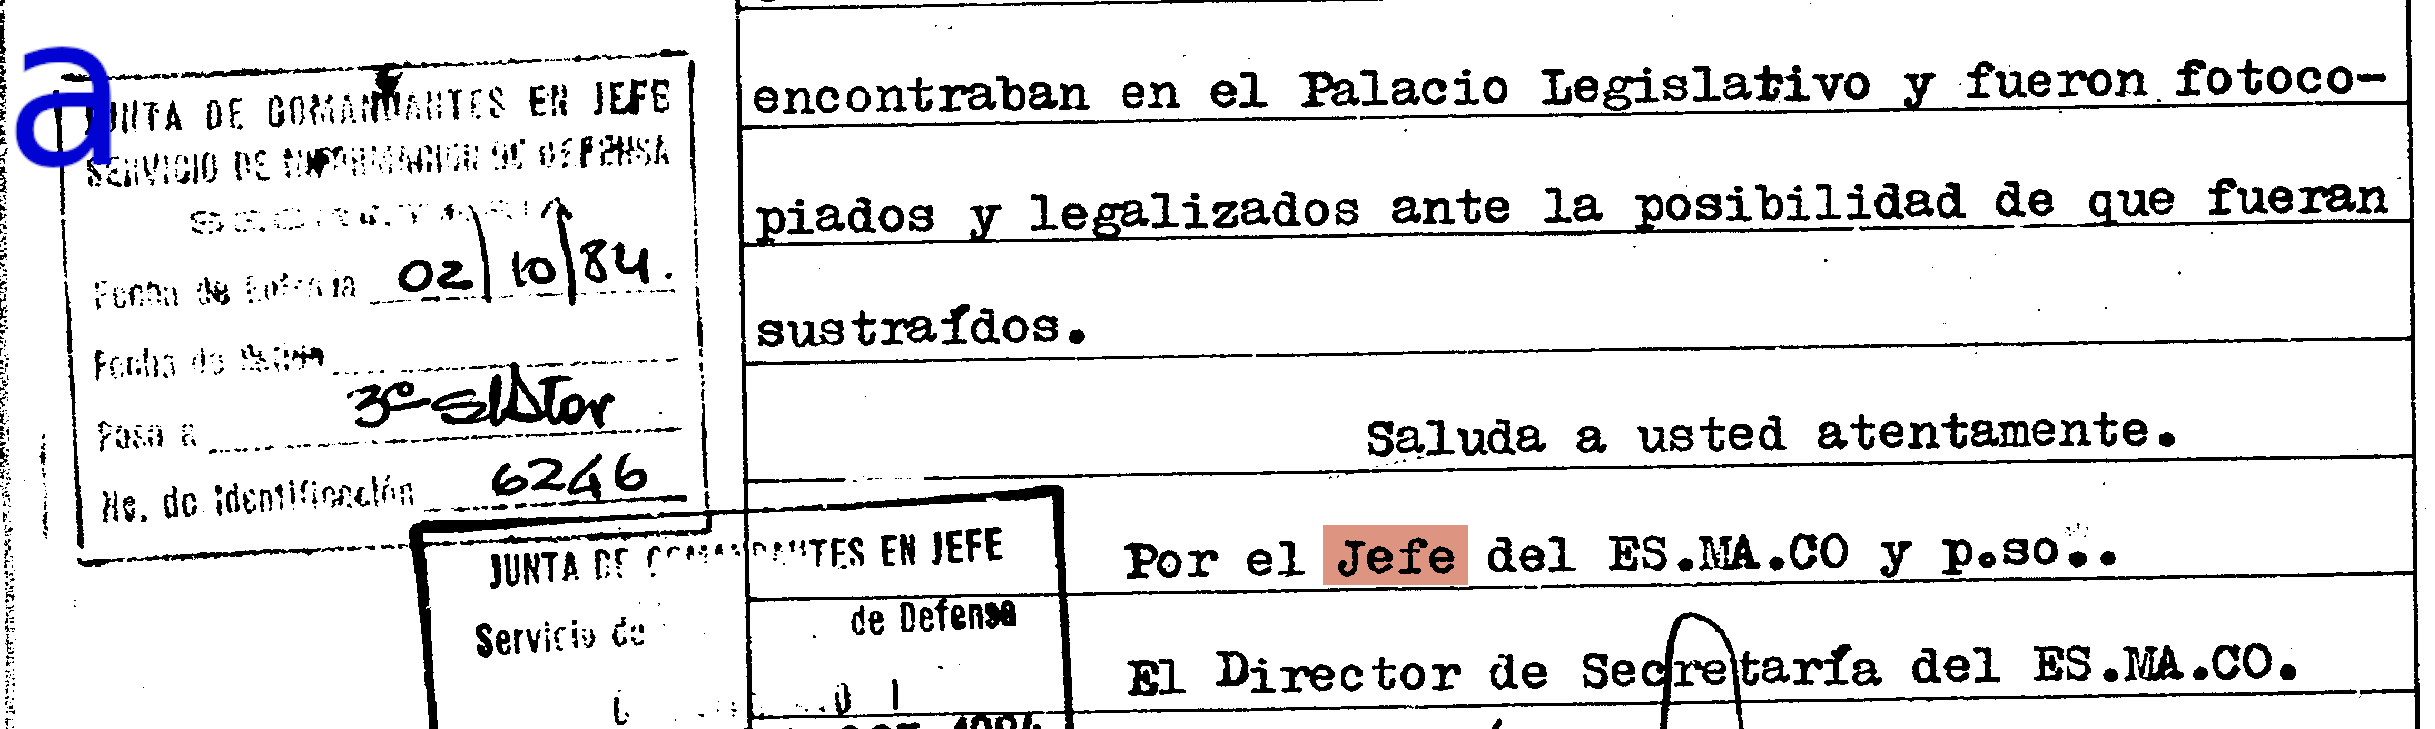
\includegraphics[width=0.85\columnwidth]{r0566_0008_crop_hl_2.png}\\[2ex]
    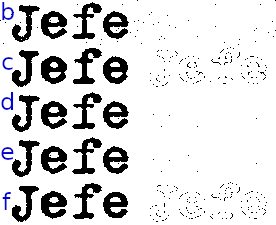
\includegraphics[width=0.85\columnwidth]{jefe2.png}
    \caption{\label{fig:visual-sim} Synthetic noise removal. Row a) detail of zoomed region. Row b) noisy (left) and error (right). Rows c--f) denoised (left) and corresponding error (right) using c) median, d) DUDE, e) Quorum, f) B-NLM.}    
\end{figure}
%
\begin{figure}
    \centering
    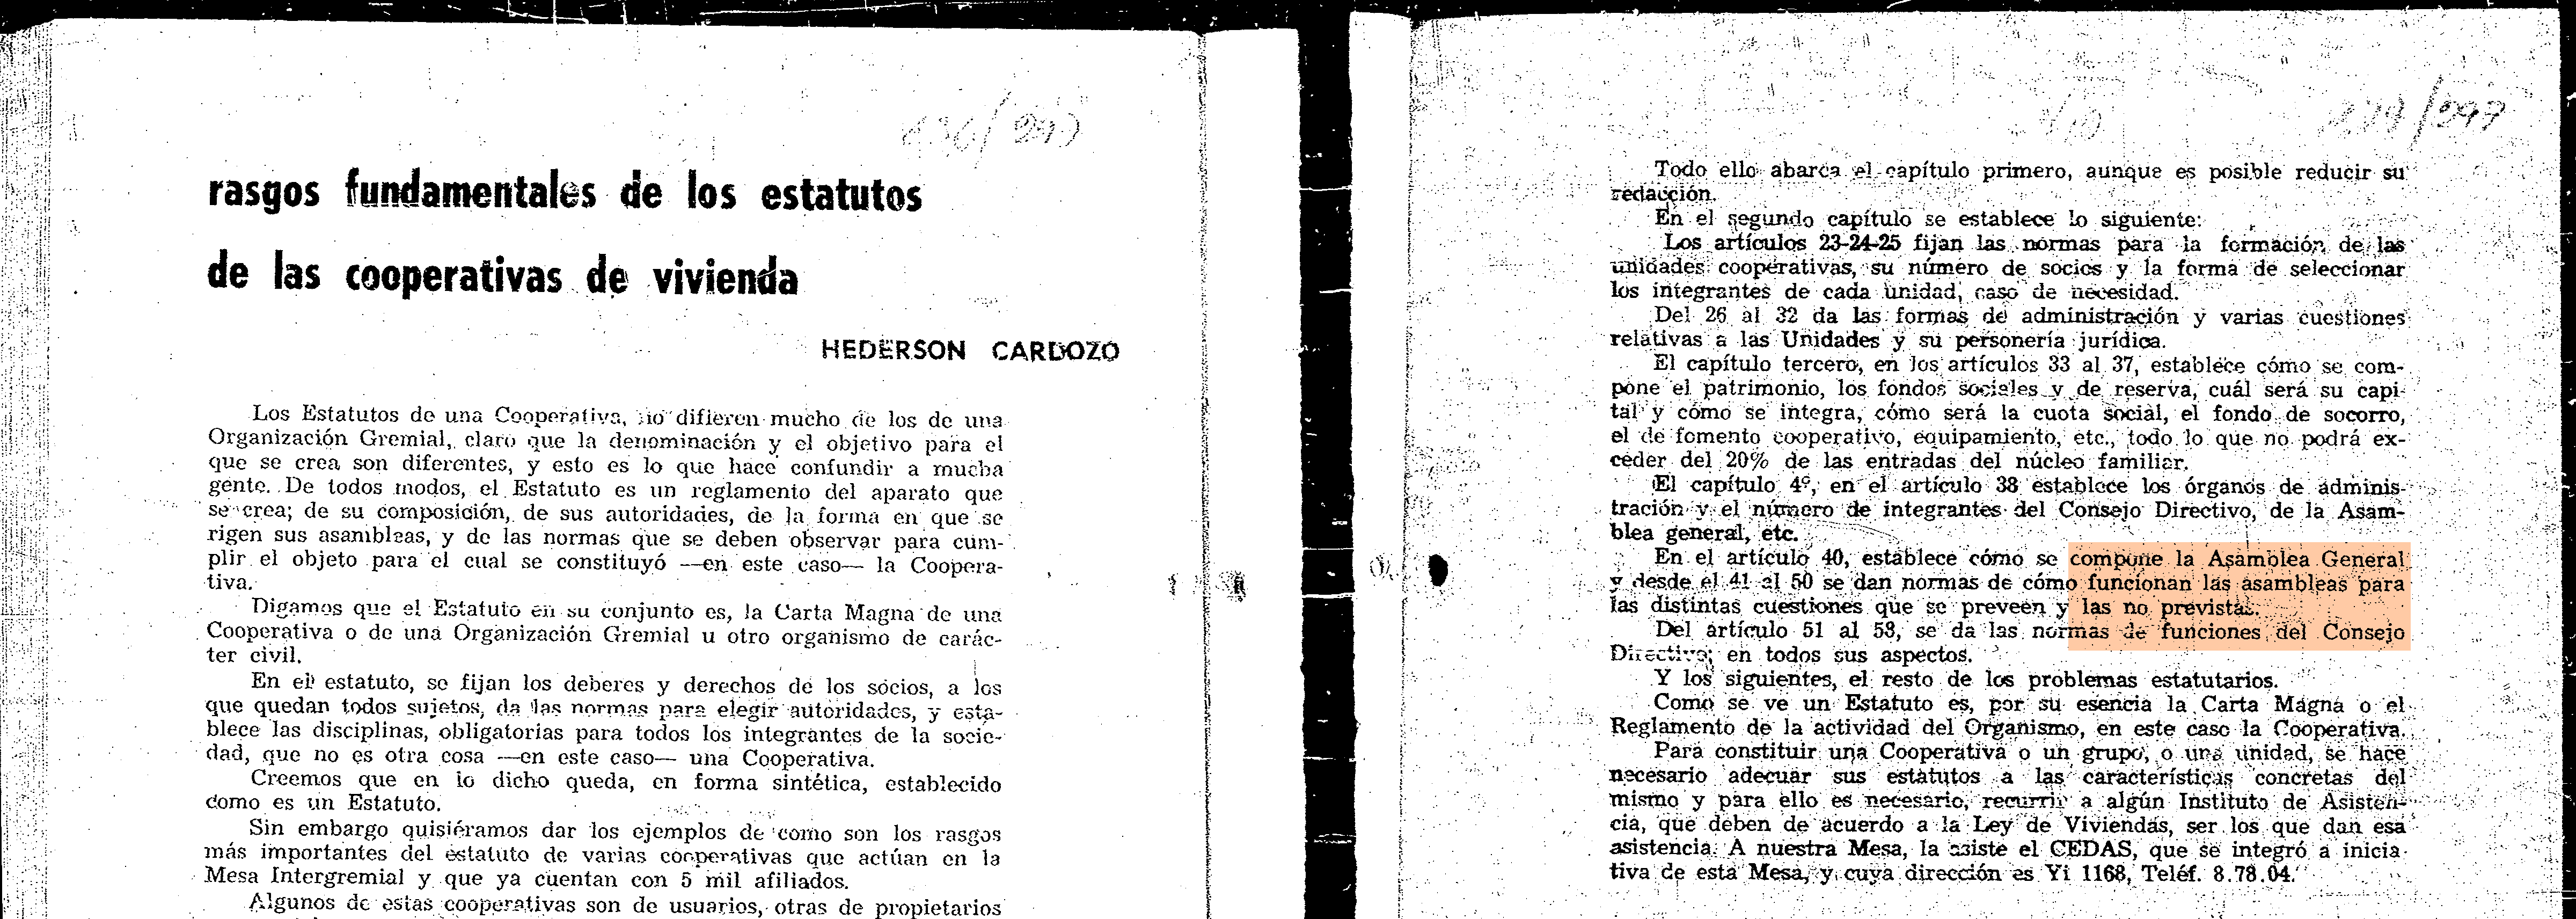
\includegraphics[width=0.9\columnwidth]{r0108_0022_crop.png}\\[2ex]
    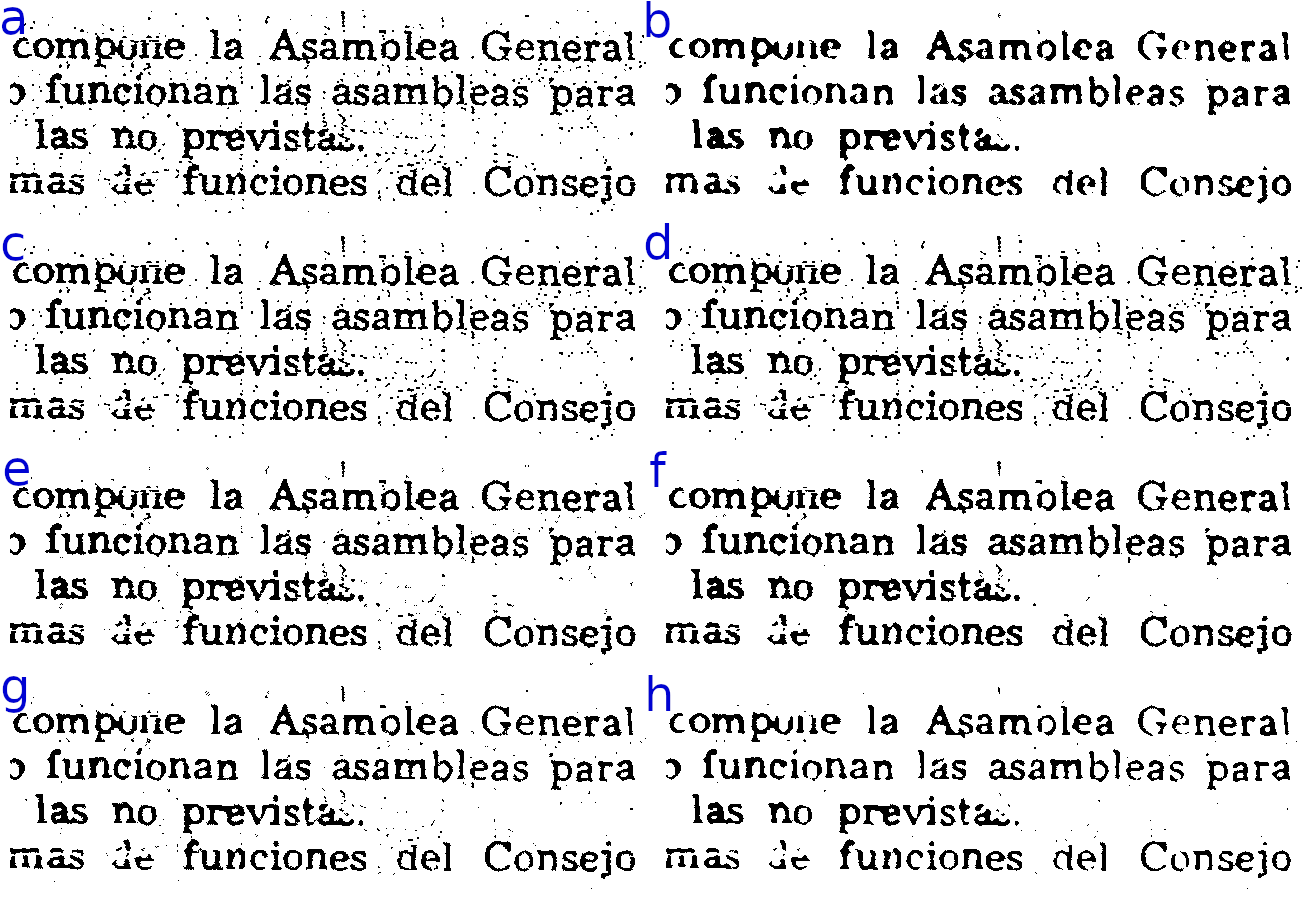
\includegraphics[width=0.9\columnwidth]{asamblea2.png}
    \caption{\label{fig:visual-real} Visual comparison of real noise removal; \emph{here $\rho$ acts as knob controlling how aggressive a denoiser will be:} top) detail of zoomed region;  a) original; b) median; c) DUDE@$\rho=10\%$; d) DUDE@$\rho=20\%$; e) Quorum@$\rho=10\%$; f) Quorum@$\rho=20\%$; g) B-NLM@$\rho=10\%$ and h) B-NLM@$\rho=20\%$ (in B-NLM, $\rho$ controls the maximum allowed distance between patches). }    
\end{figure}
%
\def\good{\color{blue}}%
\def\bad{\color{red}}%
%
\begin{table}\small
    \centering
    \caption{\label{tab:sim-noise}Results on synthetic BSC as \% of errors, for different noise levels and fixed radius of $3$ pix. ($k=24$).}
%    \begin{tabular}{c|ccccc}\hline
%        noise & median & morph. & Quorum & DUDE  & B-NLM \\\hline\hline
%        0.5\% & 0.62   & \bad 1.35   & 0.03   &  \good 0.02 & 0.82 \\
%        1.0\% & 0.62   & \bad 1.38   & 0.05   &  \good 0.04 & 0.80 \\
%        2.0\% & 0.63   & \bad 1.46   & 0.09   &  \good 0.06 & 0.77 \\
%        4.0\% & 0.65   & \bad 1.62   & 0.14   &  \good 0.10 & 0.74 \\\hline
%    \end{tabular}
    \begin{tabular}{c|cccc}\hline
        noise & median  & Quorum & DUDE  & B-NLM \\\hline\hline
        0.5\% & 0.62   & 0.03   &  \good 0.02 & \bad 0.82 \\
        1.0\% & 0.62   & 0.05   &  \good 0.04 & \bad 0.80 \\
        2.0\% & 0.63   & 0.09   &  \good 0.06 & \bad 0.77 \\
        4.0\% & 0.65   & 0.14   &  \good 0.10 & \bad 0.74 \\\hline
    \end{tabular}
\end{table}
%
\begin{table}\footnotesize
    \centering
    \caption{\label{tab:sim-size}Performance results on synthetic noise (\% of errors) for different template sizes and BSC noise with $\rho=1\%$.}
%    \begin{tabular}{c|ccccc}\hline
%        radius & median & morph. & Quorum & DUDE & B-NLM \\\hline\hline
%        1 & 0.490   & 0.255   & 0.044   &  \good 0.041 & \bad 0.807 \\
%        2 & 0.624   & \bad 1.387   & 0.051   &  \good 0.037 & 0.798 \\
%        3 & 0.874   & \bad 2.640   & 0.063   &  \good 0.041 & 0.590 \\
%        4 & 1.440   & \bad 3.580   & 0.071   &  \good 0.049 & 0.607 \\\hline
%    \end{tabular}
    \begin{tabular}{c|ccccc}\hline
        radius & k & median & Quorum & DUDE & B-NLM \\\hline\hline
        1 & 8  & 0.490   & 0.044   &  \good 0.041 & \bad 0.807 \\
        2 & 16 & 0.624   & 0.051   &  \good 0.037 & \bad 0.798 \\
        3 & 24 & \bad 0.874   & 0.063   &  \good 0.041 & 0.590 \\
        4 & 32 & \bad 1.440   & 0.071   &  \good 0.049 & 0.607 \\\hline
    \end{tabular}
\end{table}
%
\begin{table}\footnotesize
    \centering
    \caption{\label{tab:timing}Timing (in seconds) on a $3552{\times}4896$ image.}
%    \begin{tabular}{c|c|ccccc}\hline
%        radius & $k$ & median & morph. & Quorum & DUDE  & B-NLM \\\hline\hline
%        1      & 8  & \good 0.37   & 0.88   & 0.41   &  1.26 & \bad 42.60 \\
%        2      & 16 & \good 0.64   & 1.13   & 0.74   &  2.26 & \bad 44.97 \\
%        3      & 24 & \good 0.79   & 1.63   & 0.82   &  4.04 & \bad 53.17 \\
%        4      & 32 &     1.14   & 2.45   & \good 1.11   & 18.07 & \bad 49.10 \\\hline
    \begin{tabular}{c|c|cccc}\hline
        radius & $k$ & median &  Quorum & DUDE  & B-NLM \\\hline\hline
        1      & 8  & \good 0.37   & 0.41   &  1.26 & \bad 42.60 \\
        2      & 16 & \good 0.64   & 0.74   &  2.26 & \bad 44.97 \\
        3      & 24 & \good 0.79   & 0.82   &  4.04 & \bad 53.17 \\
        4      & 32 &     1.14   & \good 1.11   & 18.07 & \bad 49.10 \\\hline    \end{tabular}
\end{table}
%
\subsection{Performance on synthetic noise}

Figure~\ref{fig:visual-sim} shows our on a sample image from the dataset. This is ``clean'' image which was artificially corrupted by BSC noise with $\rho=1.0\%$, (quite high for real noisy images). Recognizable structure present in the residual images indicate that the corresponding denoiser destroyed valuable information. This is evident for Median and B-NLM, but not for DUDE and Quorum. In fact, the latter two produce almost identical results in this case, with the DUDE being  slightly better. Tables \ref{tab:sim-noise} and \ref{tab:sim-size} summarize the performance of the proposed methods for various noise levels and template sizes, together with a baseline median filter defined on the same star-shaped context. Overall, the best radius was 3 ($k=24$).

\subsection{Performance on real noise}

Figure~\ref{fig:visual-real} shows the results obtained on a sample image corrupted by real noise. Note that this noise is far from memoryless; this greatly affects the efficacy of the DUDE, which does not work well in this case. On the other hand, the Quorum denoiser seems impervious to this problem, actually standing out as the best in terms of detail preservation and noise removal. B-NLM also produces a good result, albeit being more destructive (and far more computationally expensive).

\subsection{Execution time} 
Timings are reported on Table~\ref{tab:timing}: the Quorum denoiser is almost as fast as a plain median filter, the DUDE becomes much slower for larger radii, and B-NLM is significantly slower than the rest. These results were obtained using the public implementation\footnote{\url{https://github.com/nacho-pancho/binden}} compiled using GCC 9.4.0 on an AMD Ryzen 5 3600 machine running Ubuntu 20.04/Linux 5.8.0 kernel.


\section{Concluding remarks}
We compared a number of binary denoising methods on synthetic and real noise on very large images, both in terms of execution time and quality. Two of the methods are novel and were developed specifically for this task: Quorum and B-NLM. We show that, overall, the new Quorum denoiser offers the best trade-off between quality (good or better than DUDE) and speed (almost as fast as a simple median filter).

%==================================================================================
%==================================================================================

\bibliographystyle{IEEEbib}
\balance
\bibliography{main}

%==================================================================================
\end{document}
%==================================================================================
